\documentclass{exam}

\usepackage[margin=1in]{geometry}

\usepackage{comment}
\usepackage{graphicx}
\usepackage{listings}
\usepackage{amsmath}
\usepackage{tikz}
\usetikzlibrary{matrix}
\usepackage{hyperref}
\hypersetup{colorlinks,urlcolor=blue}

\newcommand{\addend}{\text{\textsl{\color{gray}{Addend}}}}
\newcommand{\augend}{\text{\textsl{\color{gray}{Augend}}}}
\newcommand{\sumOut}{\text{\textsl{\color{gray}{Sum}}}}

\pagestyle{headandfoot}
\firstpageheader{CSCI 389}{}{Binary and C Intro Assignment}
\runningheader{CSCI 389}{}{Binary and C Intro Assignment}


\begin{document}
\title{Binary and C Intro Assignment (Evaluation)}
\author{CSCI 389: Computer Systems}
\date{Spring 2022}
\maketitle


This assignment is designed to test your understanding of binary and early c. 
Feel free to collaborate wih others and use resources, but all code and writeups must be your own. 
For submitting your code, you can convert the files to pdf (through screenshots or other methods) or provide a link to a repository or other codebase. 

\textbf{Due Date:}
Monday, February 7th at 10:00 am. 

\begin{questions}

\question[12]
\textbf{Converting Bases.}
Convert the following numbers to the specified base. 
\begin{parts}
\part[2]
Convert $93_{10}$ to binary. 
\part[2]
Convert $215_{10}$ to hexadecimal. 
\part[2]
Convert $11000101_{2}$ to decimal. 
\part[2]
Convert $1011010_{2}$ to hexadecimal. 
\part[2]
Convert $C14B_{16}$ to decimal. 
\part[2]
Convert $5A6D_{16}$ to binary. 
\end{parts}

\textbf{A.}

$\lfloor \log_{2}(93) \rfloor = 6$

$\lfloor \log_{2}(93-2^6) \rfloor = 4$

$\lfloor \log_{2}(93-2^6-2^4) \rfloor = 3$

$\lfloor \log_{2}(93-2^6-2^4-2^3) \rfloor = 2$

$\lfloor \log_{2}(93-2^6-2^4-2^3-2^2) \rfloor = 0$


$1011101$

\textbf{B.}

Number of places $\lceil \log_{16}(215)\rceil=2$

Most significant digit: $\lfloor \frac{215}{16} \rfloor = 13=D$

Least significant digit: $215-13(16)=7$

$D7$

\textbf{C.}

$2^{0}+2^{2}+2^{6}+2^{7}=197$


\textbf{D.} 

Least significant: $1010=A$

Most significant: $0101=5$

$5A$ 

\question[4]
\textbf{Binary Addition.}
Show how to add $10111001_{2}$ and $00111100_{2}$ using binary arithmetic. 

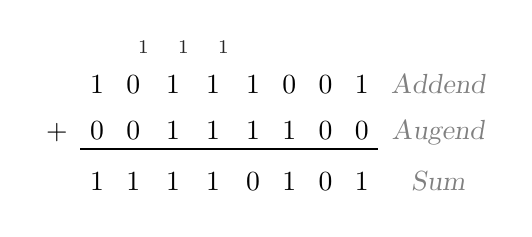
\begin{tikzpicture}[
    row 1/.style={font=\textsl,font=\scriptsize,black!85, anchor=west,
        inner sep=1.5pt},
    every node/.style={column sep=.5mm,row sep=1mm}]
    \matrix (m) [matrix of math nodes,
        nodes in empty cells,
        %nodes=draw
    ] 
    {
        &   &  1 & 1 & 1 &  &  &    &    &               \\
        & 1 & 0 & 1 & 1 & 1 & 0 & 0 & 1 &[10mm]     \addend \\
    +  & 0 & 0 & 1 & 1 & 1 & 1 & 0 & 0 &           \augend \\ 
        & 1 & 1 & 1 & 1 & 0 & 1 & 0 & 1 &           \sumOut \\                                                  
    };

    \draw[-,color=black,semithick] (m-3-2.south west) -- (m-3-9.south east);

\end{tikzpicture}

Credits to \href{https://tex.stackexchange.com/a/96764}{this} tex.stackechange post for the tikz code.

\question[4]
\textbf{Binary Multiplication.}
Show how to multiply $110100$ and $10110$ using binary arithmetic. 

\begin{equation}
\begin{array}{r}
                         110100\\
\underline{\mbox{}\times 10110}\\
                         0000000\\
                        110100\phantom{0}\\
                       110100\phantom{00}\\
                       0000000\phantom{000}\\
  \underline{\mbox{}+ 110100\phantom{0000}}\\
                     10001111000
\end{array}
\end{equation}


Credits to \href{https://tex.stackexchange.com/questions/169842/how-to-make-a-multiply-equation}{this} tex.stackexchange post for formatting.

\question[4]
\textbf{Circuits.}
Create the truth table for the following circuit:
\begin{center}
\includegraphics[width=0.6\textwidth{}]{circut.png}
\end{center}

$\begin{array}{|c c c | c|}
x&y&z&output\\
1&1&1&1\\
1&1&0&0\\
1&0&1&0\\ % by bottom
1&0&0&1\\ % by bottom
0&1&1&1\\ % by middle
0&1&0&1\\
0&0&1&0\\ % by top
0&0&0&0
\end{array}$

\question[16]
\textbf{Galaxy Explorers (C).}

Congratulations! you are now the big-shot CTO of Masstronaut, Inc., a hot new startup developing the next massive multiplayer space exploration game, "Galaxy Explorers".

The current prototype is implemented in Python in the file \texttt{update\_locations.py} available on Moodle, 
but this prototype turns out to scale poorly to many players. 
After some profiling, you realize that one of the slowest pieces of code in your game server is the one that updates the position of all of the objects in 3D space, every turn: spaceships, planets, asteroids, space junk, astronauts taking a space walk, you name it. 

\begin{parts}
\part[5]
\textbf{Benchmarking.}
You'll start with a micro-benchmark in Python that encapsulates the code that updates locations (see \texttt{update\_locations.py}). 
This benchmark takes two parameters: the number of objects in space, and how many iterations (game turns) to simulate. 
It updates all objects every turn, and measures the mean time to update a single coordinate. 
Your first task is to understand the scaling properties of this code.

Run this code for multiple object counts (say from 28 to 224 in powers of two). 
For a small number of objects, you'll need to run for many iterations (turns) to get a statistically stable measurement. 
For larger objects, many turns would take too long, and may not be necessary. 
But you'll probably still see some variation from run to run. 
Once you decide on good choices for the number of iterations, run the benchmark for all these sizes and collect the results. 
Note that the checksum printed should remain the same between consecutive runs with the same arguments (as a sanity check). 

%Provide a brief summary of your results that you believe captures the essence of the information. 
Plot a line graph of mean update time per coordinate as a function of total number of objects (first parameter). 
Explain what you chose as your testing parameters and how you chose them. 
If you're using a script or modified python file, submit that on gradescope.
There is no single correct answer here, I just want to see your reasoning.

\part[8]
\textbf{Port to C.}
Port this benchmark to C, as closely as possible to the Python version. 
You may use any standard library functions. 
Repeat the above measurements and create a new graph that adds the C line to the Python line.

You may find that you can run many more iterations now, and perhaps larger object counts. 
Explain any parameter changes you make and demonstrate how it's better (or worse) than before.

To time a function in C, you can use \texttt{clock\_gettime} (with the \texttt{CLOCK\_MONOTONIC} argument). 
Since you're using a different random number generator now, you'll probably have different initial values and therefore a different checksum than the Python version. 
That's fine, as long as you're getting the same checksum from run to run.

\part[3]
\textbf{Comparing Types.}
Compare your C implementation using different C types: float, double, int8\_t, int16\_t, int32\_t, int64\_t for the coordinate and velocity types in terms of performance. 
Report your findings.

Note: the checksum will probably not be computed correctly for the integral types due to precision loss. That's OK, though: we're only interested in the performance trade-offs.
\end{parts}
\end{questions}


\textbf{A.}

Iterations were set to 1,000

\begin{center}
\begin{tabular}{||c | c c c|  c c ||} 
 \hline
 Size & Trial 1 & Trial 2 & Trial 3 & \texttt{checksum} & avg time\\ [0.5ex] 
 \hline\hline
1 & $0.4276000108802691$ & $0.7721000001765788$ & $0.42749999556690454$ & $-108.86444470728384$ & $0.5424000022$ \\ 
 \hline
10 & $0.20790999988093972$ & $0.21666000102413818$ & $0.20232999959262088$ & $217.4809655065676$ & $0.20896666683$ \\ 
 \hline
100 & $0.17177300003822893$ & $0.16994999998132698$ & $0.25543299998389557$ & $2578.8360260324353$ & $0.199052$ \\ 
 \hline
1000 & $0.17516680000699125$ & $0.20967949999612756$  & $0.2134689999948023$  & $-3247.4138201922724$ & $0.19943843333$\\ [1ex] 
 \hline
\end{tabular}
\end{center}


\textbf{B.} Check out my \href{https://github.com/Goodernews/CS-389-Systems/tree/main/HW\%202}{github repo} for the code


\textbf{C.}

All trials were size \texttt{1000} and iters \texttt{1000}.

\textit{I could have written a bash script to compute this, but I did not feel up to it}

\begin{center}
\begin{tabular}{||c | c c c|  c c ||} 
 \hline
 Type & Trial 1 & Trial 2 & Trial 3 & \texttt{checksum} & avg time\\ [0.5ex] 
 \hline\hline
 float\_t & $0.142010$ & $0.142610$ & $0.071460$ & $-1412662.000000$ & $0.11869333$ \\ 
 \hline
  double & $0.142980$ & $0.146740$ & $0.158410$ & $ -1412662.000000$ & $0.14937666$ \\ 
 \hline
 int8\_t & $0.118020$ & $0.156070$ & $0.134660$ & $-54$ & $0.13625$ \\ 
 \hline
 int16\_t & $0.137480$ & $0.142270$ & $0.111910$  & $29130$ & $0.13055333$\\
 \hline
 int32\_t & $0.082340$ & $0.139090$ & $0.145590$ & $-1412662$ & $0.12234$ \\
 \hline
int64\_t & $0.140290$ & $0.152290$ & $0.139420$ & $-1412662$ & $0.144$ \\ [1ex] 
 \hline
\end{tabular}
\end{center}



\end{document}